\chapter{El problema de los dos cuerpos}

\begin{miparrafo}
Problema de los dos cuerpos

En mecánica, el problema de los dos cuerpos consiste en determinar el movimiento de dos partículas puntuales que solo interactúan entre sí. Los ejemplos comunes incluyen la Luna orbitando la Tierra y en ausencia del Sol, es decir aislados, un planeta orbitando una estrella, dos estrellas que giran en torno al centro de masas (estrella binaria), y un electrón orbitando en torno a un núcleo atómico. 

Como veremos en el tema, las leyes de Newton nos permite reducir el problema de dos-cuerpos a un problema de un-cuerpo equivalente, es decir, a resolver el movimiento de una partícula sometida a un campo gravitatorio conservativo y que por tanto deriva de un potencial externo.  El problema puede resolverse exactamente, por el contrario, el problema de los tres cuerpos (y, más generalmente, el problema de n$n$ cuerpos con $n\geq 3$) no puede resolverse, excepto en casos especiales.	
\end{miparrafo}

\section[El problema de los dos cuerpos. Masa reducida]{El problema de los dos cuerpos. Masa reducida\sectionmark{Problema 2 cuerpos. Masa reducida}}
\sectionmark{Problema 2 cuerpos. Masa reducida}

\begin{multicols}{2}
Consideremos dos cuerpos que ejercen fuerzas entre sí y, además, están inmersos en un campo exterior a ellos.

Tercera de Newton: $\ \vec F_{12}=-\vec F_{21}$

Posiciones: $\vec r_{12}=\vec r_1- \vec r_2$

\begin{figure}[H]
	\centering
	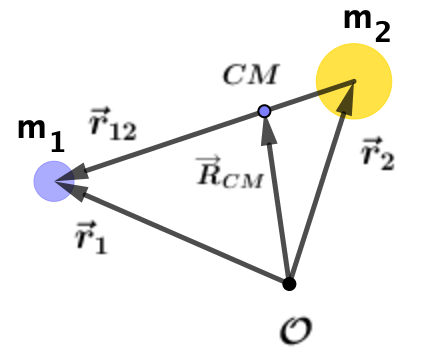
\includegraphics[width=.4\textwidth]{imagenes/imagenes13/T13IM01.png}
\end{figure}
\end{multicols}
Nuestro objetivo va a ser encontrar las ecuaciones de movimiento que rigen el sistema de los dos cuerpos como tal y que hacen que se muevan como un ente.

Cada uno de los dos cuerpos, por separado:
$ \quad \begin{cases}
 \displaystyle \ m_1 \ \dv{\vec v_1}{t} = \vec F_{12}+\vec F_1^{(e)} \\ \\	 
 \displaystyle \ m_2 \ \dv{\vec v_2}{t} = \vec F_{21}+\vec F_2^{(e)}
 \end{cases}$
 
 Vamos a intentar refundir estas dos ecuaciones de movimiento en una sola.

Para ello, consideremos:
$ \quad \begin{cases}
 \displaystyle \overrightarrow {R}_{CM}=\dfrac {m_1 \vec r_1+m_2 \vec r_2}{m_1+m_2} \\ 
 \displaystyle \vec r_{12}=\vec r_1-\vec r_2
 \end{cases}$

Despejando de aquí $\vec r_1$ y $\vec r_2$,
$\ \  \vec r_1=\dfrac {m_1+m_2}{m_1} \vec R_{CM}-\dfrac {m_2}{m_1}\vec r_2; \ \  \vec r_2=\vec r_1-\vec r_{12}$

\small{$\vec r_1=\dfrac {m_1+m_2}{m_1} \vec R_{CM}-\dfrac {m_2}{m_1}\vec r_1+\dfrac{m_2}{m_1}\vec r_{12} \to \vec r_1\left( 1+\dfrac {m_2}{m_1} \right) =\dfrac{m_1+m_2}{m_2}\vec R_{CM} +\dfrac{m_2}{m_1}\vec r_{12}$}

\normalsize{Finalmente,} obtenemos el siguiente \emph{cambio de coordenadas}:

$$ \vec r_1 = \overrightarrow {R}_{CM}\ + \ \dfrac{m_2}{m_1+m_2}\ \vec r_{12} \qquad \qquad \vec r_2 = \overrightarrow {R}_{CM}\ + \ \dfrac{m_1}{m_1+m_2}\ \vec r_{12}$$

Tenemos las ecuaciones de movimiento de cada partícula por separado, tenemos la tercera de Newton y este cambio de coordenadas. Con todo esto vamos a hacer un \emph{truco matemático} \textbf{sumando} las ecuaciones de movimiento de los cuerpos independientes.

$\displaystyle m_1 \dv{\vec v_1}{t}+m_2 \dv{\vec v_2}{t} = \vec F_1^{(e)}+\vec F_2^{(e)}+\cancel{\vec F_{12}}+\cancel{\vec F_{21}}$

Suponiendo que las masas son constantes, $\displaystyle \dv{m_i}{t}=0$ y derivando respecto del tiempo el vector de posición del $CM$,

$\displaystyle \dv{\overrightarrow R_{CM}}{t}=\dfrac 1{m_1+m_2} \left( m_1 \dv{\vec r_1}{t} + m_2 \dv{\vec r_2}{t} \right)=\dfrac 1{m_1+m_2}(m_1\vec v_1+m_2 \vec v_2)$

Volviendo a derivar respecto al tiempo,

\small{$\displaystyle \dv[2]{\overrightarrow {R}_{CM}}{t}=\dfrac 1 {m_1+m_2} \left( m_1 \dv{\vec v_1}{t} + m_2\dv{\vec v_2}{t} \right)=\dfrac 1 {m_1+m_2} \left(\vec F_1^{(e)}+\vec F_2^{(e)}\right)=\dfrac{\vec F^{(e)}}{m_1+m_2}$}

\normalsize{Finalmente,} obtenemos una ecuación de movimiento que unifica a los dos cuerpos:

\begin{equation}
\subrayado{\boldsymbol{
(m_1+m_2) \ \dv[2]{\overrightarrow {R}_{CM} }{t}	 \ = \ \overrightarrow F^{(e)}
}}
\end{equation}

\begin{miparrafodestacado}
Ecuación de movimiento del sistema donde la masa es la masa total del sistema, el vector de posición es el del centro de masas y la fuerza externa que actúa es la que actúa sobre el centro de masas.	
\end{miparrafodestacado}

\textbf{Restando}, ahora, las dos ecuaciones de movimiento de los dos cuerpos por separado:

$m_1 m_2 \ \displaystyle \left( \dv{\vec v_1}{t} - \dv{\vec v_2}{t} \right) \ = \ m_2 \vec F_{12} \ - \  m_1 \vec F_{21}\ + \ m_2 \vec F_1^{(e)} \ - \ m_1 \vec F_2^{(e)} \ = \quad (m_1+m_2) \vec F_{12} + m_2 \vec F_1^{(e)}-m_1 \vec F_2^{(e)}$

$\vec r_{12}=\vec r_1 - \vec r_2 \ \to \ \displaystyle \dv{\vec r_{12}}{t}=\dv{\vec r_1}{t}-\dv{\vec r_2}{t} \ \to \  \dv[2]{\vec r_{12}}{t}=\dv{\vec v_1}{t}-\dv{\vec v_2}{t}$

$m_1 m_2 \ \displaystyle \left( \dv{\vec v_1}{t} - \dv{\vec v_2}{t} \right) \ =m_1m_2 \dv[2]{\vec r_{12}}{t}= (m_1+m_2) \vec F_{12}+ m_2\vec F_1^{(e)}-m_1\vec F_a^{(e)}$

$\displaystyle m_1m_2 \dv[2]{\vec r_{12}}{t}= (m_1+m_2) \vec F_{12}+ m_1m_2 \left( \dfrac {\vec F_1^{(e)}}{m_1}-  \dfrac {\vec F_2^{(e)}}{m_2} \right)$

Como caso particular, exigimos que $\dfrac{\vec F_i^{(e)}}{m_i}=\overrightarrow{cte},\quad i=1,2$ con lo que el último paréntesis anterior será cero. Esto significa que la aceleración es un vector constante, relación común en muchos campos de la física.

$\displaystyle \dfrac{m_1m_2}{m_1+m_2}\  \dv[2]{\vec r_{12}}{t}= \vec F_{12} \to \ \mu \  \dv[2]{\vec r_{12}}{t}= \vec F_{12}, \ \ con \ \ \mu=\dfrac{m_1m_2}{m_1+m_2}$, 

donde $\mu$ es la llamada \emph{masa reducida} del sistema.

\begin{equation}
\subrayado{\boldsymbol{
 \mu \  \dv[2]{\vec r_{12}}{t}= \vec F_{12}
}}
\end{equation}

\begin{miparrafodestacado}
	El movimiento relativo de dos partículas sujetas a una interacción mutua y a un campo exterior	que satisface la relación $\vec F/m=\overrightarrow{cte}$ es equivalente al movimiento de una  partícula cuya masa sea la masa relativa del sistema y sometida a una fuerza igual a la fuerza medida por un observador inercial.
\end{miparrafodestacado}

El sistema Tierra-Luna, p.e., puede ser estudiado con las dos ecuaciones siguientes, donde hemos llamado $M=m_1+m_2$ a la masa total del sistema.

\begin{equation}
\subrayado{
\boldsymbol{ \boxed{\ 
\begin{cases}
\quad \displaystyle 	\mu \  \dv[2]{\vec r_{12}}{t} &= \vec F_{12} \\
\quad \displaystyle   M \ \dv[2]{\overrightarrow {R}_{CM} }{t}	 \ &= \ \overrightarrow F^{(e)}
\end{cases}\ } }
}
\end{equation}

Análisis de la masa reducida:
$\quad \mu=\dfrac{m_1m_2}{m_1+m_2}=\dfrac{m_1}{1+\dfrac{m_1}{m_2}}$

Usando el conocido desarrollo es serie de Maclaurin: $\ \dfrac 1{1+x} \ \underset {x\to 0}{=} \  1-x$, podemos escribir:

\begin{table}[H]
\begin{tabular}{lll}
$\quad \text{si }\ m_1<<m_2$  &$\to$&$\mu \ = \ m_1 \left( 1-\dfrac{m_1}{m_2} 	\right)$ \\
$\quad \text{si }\ m_1<<<m_2$ &$\to$&$\mu \ = \ m_1 	$
\end{tabular}
\end{table}

$\text{si }\ m_1=m_2 \to \mu \ = \ \dfrac{m^2}{2m} \ = \ \dfrac{m}{2},\   $ por ejemplo, para el caso de protón y neutrón dentro del $\ _1^2H\ $ (Deuterio).

\section[Energía, cantidad de movimiento y momento angular respecto al CM en el problema de los dos cuerpos]{Energía, cantidad de movimiento y momento angular respecto al CM en el problema de los dos cuerpos\sectionmark{Magnitudes en CM problema dos cuerpos}}
\sectionmark{Magnitudes en CM problema dos cuerpos}

Situamos el origen $\mathcal O$ del sistema de referencia en el $CM$, evidentemente ocurrirá que: $\quad \boldsymbol {\overrightarrow{R}_{CM}=\vec 0}$

\textbf{------ Energía}: $\ E=\mathcal E_c+\mathcal E_{p,int} + \mathcal E_p^{(e)}$

En el caso del problema de los dos cuerpos:

$\mathcal E_c=\sum_i \dfrac 1 2 m_i v_{i,CM}^2+\dfrac 1 2 M \cancelto{0}{v_{CM}^2}=\dfrac 1 2 m_1 v_{1,CM}^2 +\dfrac 1 2 m_2 v_{2,CM}^2$

Por otro lado:

$\vec r_1=\cancelto{0}{\vec R_{CM}}+\dfrac{m_2}{m_1+m_2}\vec r_{12}; \qquad \qquad \vec r_2=\cancelto{0}{\vec R_{CM}}+\dfrac{m_1}{m_1+m_2}\vec r_{12}$

Derivando:

$\vec v_{1,CM}=\dfrac {m_2}{m_1+m_2}\ vec v_{12}; \qquad \qquad \vec v_{2,CM}=\dfrac {m_1}{m_1+m_2}\ vec v_{12}$

Sustituyendo en la $\ \mathcal E_c$:

\small{$\mathcal E_c= \dfrac 1 2 \left( \dfrac {m_1m_2^2}{(m_1+m_2)^2}\ v_{12}^2+  \dfrac {m_1^2m_2}{(m_1+m_2)^2}\ v_{12}^2  \right) = \dfrac 1 2 \ \dfrac{m_1m_2}{(m_1+m^2)^{\cancel{}2}}\ \cancel{(m_1+m_2)} \ v_{12}^2$}
 
 \normalsize{Luego,}
 
 \begin{equation}
 \boldsymbol{ \mathcal E_c \ = \ \dfrac 1 2 \ \mu \ v_{12}^2	 }
 \end{equation}

Energía cinética de los dos cuerpos en el sistema $CM$, $\mu$ es la masa reducida y $v_{12}$ la velocidad relativa de una partícula respecto a la otra.

Si las fuerza son conservativas, la energía potencial no es función del origen de coordenadas.

\textbf{------ Cantidad de movimiento:}

$\overrightarrow R_{CM}=0=\dfrac{m_1 \vec r_1 + m_2 \vec r_2}{m_1+m_2} \ \to \ m_1 \vec r_1 + m_2 \vec r_2=0$. 

Derivando respecto al tiempo:

\begin{equation}
\boldsymbol{
m_1 \ \vec v_{1,CM }\ = - \ m_2 \ \vec v_{2,CM}
}	
\end{equation}

La cantidad de movimiento sigue conservándose en el problema de los dos cuerpos y en el sistema centro de masas.

\textbf{------ Momento angular:}

El teorema de König, $\overrightarrow L=\overrightarrow R_{CM}\times M \vec V_{CM}+\sum_i \vec r_{i,CM} \times m_i \vec V_{i,CM}$, en nuestro caso: \textcolor{gris}{($\vec R_{CM}=0$)}

$\overrightarrow L =  \vec r_{1,CM} \times m_1 \vec V_{1,CM} +  \vec r_{2,CM} \times m_2 \vec V_{2,CM}$. 

Sustituyendo los $\vec r_i$ en función de $\vec r_{12}$ y $\vec R_{CM}$

$\overrightarrow L = \left( \dfrac{m_2}{m_1+m_2}\vec r_{12}\right) \times m_1 \left( \dfrac {m_2}{m_1+m_2} \vec v_{12}\right) \ + \ 
\left( \dfrac{m_1}{m_1+m_2}\vec r_{12}\right) \times m_2 \left( \dfrac {m_1}{m_1+m_2} \vec v_{12}\right)$


\small{$\overrightarrow L =  \dfrac{m_1m_2^2}{(m_1+m_2)^2} \ ( \vec r_{12} \times \vec v_{12} )  +   \dfrac{m_1^2m_2}{(m_1+m_2)^2} \ ( \vec r_{12} \times \vec v_{12} ) $}

\normalsize{$\overrightarrow L = \dfrac{m_1m_2\cancel{(m_1+m_2)}}{(m_1+m_2)^{\cancel{2}}} \ ( \vec r_{12} \times \vec v_{12} ) $}

\begin{equation}
\boldsymbol{
\overrightarrow L \ = \ \vec r_{12} \ \times \  \mu \ \vec v_{12}
}	
\end{equation}

El momento angular del sistema de los dos cuerpos en el sistema de referencia $CM$ es igual al producto vectorial del vector de posición relativo por la masa reducida y la velocidad relativa.

\section{Ley de las áreas}


Observador situado en el $CM$

Th. momento angular: $\displaystyle \dv{\overrightarrow L}{t}=\overrightarrow M^{(e)}$.
En nuestro caso: $\overrightarrow M^{(e)}=\sum_i \vec r_i \times \vec F_i^{e}$

$\displaystyle \dv{\overrightarrow L}{t}=\vec r_1 \times \vec F_1^{(e)} + \vec r_2 \times \vec F_2^{(e)} $
\begin{multicols}{2}
$ \vec r_1 = \overrightarrow {R}_{CM}\ + \ \dfrac{m_2}{m_1+m_2}\ \vec r_{12}$

$\vec r_2 = \overrightarrow {R}_{CM}\ + \ \dfrac{m_1}{m_1+m_2}\ \vec r_{12}$

$\quad$

Observador $\mathcal O$ situado en $CM$:

$\overrightarrow R_{CM}=0$
\begin{figure}[H]
	\centering
	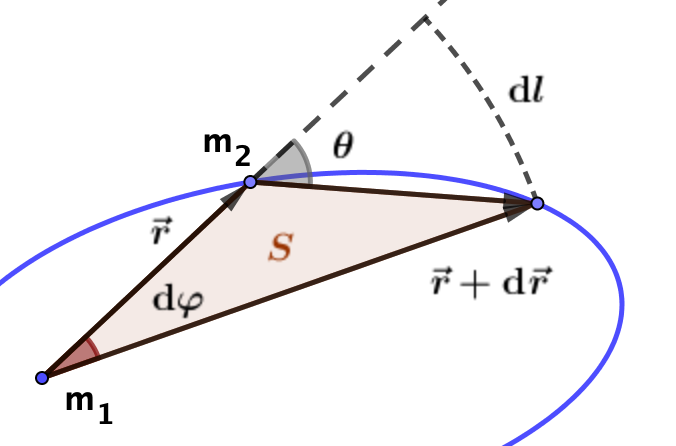
\includegraphics[width=.5\textwidth]{imagenes/imagenes13/T13IM02.png}
\end{figure}
\end{multicols}

$\displaystyle \dv{\vec L}{t}=\dfrac{m_2}{m_1+m_2}\vec r_{12}\times \vec F_1^{(e)}-\dfrac{m_1}{m_1+m_2}\vec r_{12}\times \vec F_2^{(e)}$

$\displaystyle \dv{\vec L}{t}=\mu \vec r_{12} \times \left( \dfrac {\vec F_1^{(e)}}{m_1} - \dfrac {\vec F_2^{(e)}}{m_2} \right)$

Exigiendo, de nuevo, que $\dfrac {\vec F^{(e)}}{m}=\overrightarrow{cte}$, el paréntesis anterior se anula, entonces:

\begin{equation}
\dv{\overrightarrow L}{t}=\vec 0 \quad \to \quad \subrayado{ \ \boldsymbol{ \overrightarrow   L=\overrightarrow {cte}} \ }  
\end{equation}

\begin{miparrafodestacado}
El momento angular es un vector constante, luego los vectores $\vec r_{12}$ y $\vec v_{12}$ están siempre en un plano, \emph{la órbita es única}.
\end{miparrafodestacado}

Sabemos que para movimientos en un plano, órbitas circulares o elípticas, son mejores las coordenadas polares: $\vec r_{12},\ \theta$.

Como vimos en cinemática, en la ecuación \ref{veloc-polares} (velocidad en polares),

$$\displaystyle \vec v_{12}\ =\ \dv{\vec r_{12}}{t} \ \vec u_{r_{12}} \ + \  \vec r_{12} \ \dv{\theta}{t} \ \vec u_{\theta}$$

Vamos a eliminar los subíndices pero hemos de recordar que estamos en movimiento relativo.


$\vec v=\displaystyle \dv{r}{t} \vec u_r + r \dv{\theta}{t} \vec u_{\theta}; \quad \vec L=\vec r \times \mu \vec v \quad \to$
$\quad \displaystyle \vec L = \vec r \times \mu \left(  \dv{r}{t} \vec u_r + r \dv{\theta}{t} \vec u_{\theta} \right) $ 

\textcolor{gris}{$(\vec r \times \vec u_r=0)$}; $\ \vec r=r\vec u_r \ \to \ \vec L=\displaystyle 
\mu r \dv{\theta}{t} \left( \vec r \times \vec u_\theta \right)=
\mu r^2 \dv{\theta}{t}  \left( \vec u_r \times \vec u_\theta  \right) $

$\vec u_r \times \vec u_\theta=\vec u_p$, perpendicular a ambos vectores.

$\displaystyle \vec L =\mu r^2 \dv{\theta}{t} \vec u_p \ \to \ L=\mu r^2 \dv{\theta}{t} \ \Rightarrow $

\begin{equation}
\label{ele-mu}
\subrayado{ \ \boldsymbol{r^2 \ \dv{\theta}{t}=\dfrac L \mu} \ }
\end{equation}

Como $\dfrac L \mu$ es una constante del movimiento, $\boldsymbol{r^2 \ \dv{\theta}{t}}$ ha de ser una \textbf{constante del movimiento.}

El área barrida es el área del sector de radio $r$ \textcolor{gris}{($r+\dd  r \approx \dd r$)} y ángulo $\theta$ \textcolor{gris}{en radianes} es: $\dd S = \frac 1 2 \theta r^2$.

Derivando respecto al tiempo, $\displaystyle \ \boldsymbol{\dv{S}{t}}=\dfrac 1 2 r^2 \dv{\theta}{t}= \dfrac{L}{2\mu}=\boldsymbol{cte}$, una constante del movimiento.

\begin{miparrafodestacado}
\emph{El radiovector barre áreas iguales en tiempos iguales} (segunda ley de Keppler).	
\end{miparrafodestacado}




\newpage %******************************************************
\begin{myblock}{El problema de los $n$ cuerpos}

\vspace{2mm} Se trata de un problema matemático originado en un modelo físico para explicar el movimiento de los astros en el sistema solar. Éste ha sido paradigmático para la ciencia desde la antigüedad hasta nuestros días. Las técnicas, que ingeniosamente desarrollaron célebres científicos a lo largo de la historia para abordar el problema, se revelaron extremadamente fructíferas para el estudio de la mayoría de los modelos matemáticos provenientes de otras disciplinas. Sin embargo, estos numerosos científicos, entre quienes podemos citar a Isaac Newton, Leonard Euler, Lagrange, Weierestrass, Hamilton, Jacobi, Poincaré, Kolmogorov, Lyaponov, no lograron dar una solución satisfactoria al problema original que consiste en predecir la evolución final de las trayectorias de los astros. 

\vspace{2mm} El problema físico puede formularse, informalmente, de la siguiente manera: dadas en un instante las posiciones y las velocidades de dos o más partículas que se mueven bajo la acción de sus atracciones gravitatorias mutuas, siendo conocidas las masas de las partículas, calcular sus posiciones y velocidades para otro instante. 

\vspace{2mm} En la actualidad, sólo se conocen algunos resultados particulares dependiendo del valor de $n$.	

\begin{figure}[H]
	\centering
	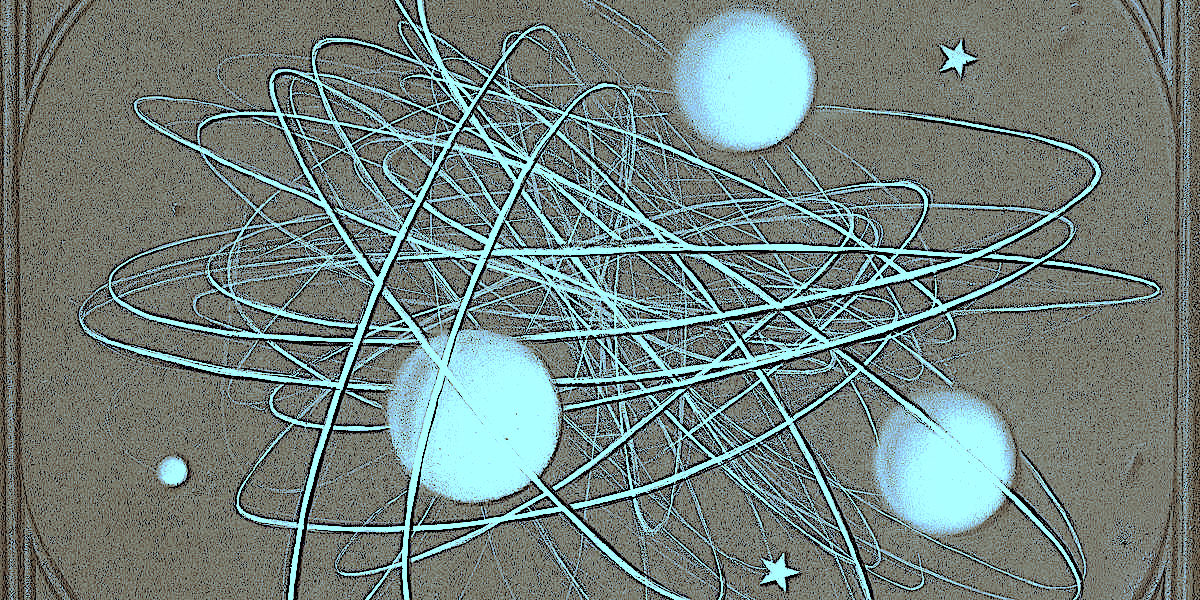
\includegraphics[width=1\textwidth]{imagenes/imagenes13/T13IM03.png}
\end{figure}
\end{myblock}
